\documentclass[a4paper,12pt]{article}

\usepackage{mystyle}

\usepackage{gensymb}
\usepackage{scalerel}
\usepackage{stackengine}

% https://tex.stackexchange.com/questions/86238/searching-for-up-and-down-arrow-symbol
% \usepackage{mathabx}  % All breaks if import this...

\DeclareMathOperator{\upups}{\uparrow\!\uparrow}
\DeclareMathOperator{\updowns}{\uparrow\!\downarrow}


% https://tex.stackexchange.com/questions/595/how-can-i-get-bold-math-symbols
% \usepackage{bm}  % XeTeX breaks with this...

% \usepackage{skull}  % skull
\usepackage{halloweenmath}  % \bigpumpkin, skull (https://tug.ctan.org/info/symbols/comprehensive/symbols-a4.pdf -- Table 76)

\usepackage{tikzsymbols}

% https://tex.stackexchange.com/questions/3266/how-do-i-use-a-circle-as-a-math-accent-larger-than-mathring
% https://tex.stackexchange.com/a/3270/135045
\usepackage{accents}

\renewcommand{\mathring}[1]{\accentset{\circ}{#1}}


% https://www.overleaf.com/learn/latex/Typesetting_quotations#epigraph_package
\usepackage{epigraph}

\setlength{\epigraphrule}{0pt}


\graphicspath{ {images/} }


% https://tex.stackexchange.com/questions/5461/is-it-possible-to-change-the-size-of-an-arrowhead-in-tikz-pgf
\usetikzlibrary{arrows.meta}


\DeclareMathOperator{\Image}{Im}

\definecolor{pink}{RGB}{218, 3, 174}
\definecolor{violet}{RGB}{148, 0, 211}
\definecolor{green}{RGB}{0, 153, 0}
\definecolor{orange}{RGB}{255, 153, 0}
\definecolor{blue}{RGB}{5, 73, 255}
\definecolor{cyan}{RGB}{31, 206, 203}
\definecolor{cyan2}{RGB}{0, 166, 147}
\definecolor{cyangreen}{RGB}{0, 155, 118}
\definecolor{cyangreen2}{RGB}{0, 109, 91}

\definecolor{yellow}{RGB}{255, 179, 0}
\definecolor{red}{RGB}{246, 74, 70}
\definecolor{grey}{RGB}{220, 220, 220}


% https://tex.stackexchange.com/a/101138/135045

\newcommand\widesim[1]{\ThisStyle{%
  \setbox0=\hbox{$\SavedStyle#1$}%
  \stackengine{-.1\LMpt}{$\SavedStyle#1$}{%
    \stretchto{\scaleto{\SavedStyle\mkern.2mu\sim}{.5150\wd0}}{.6\ht0}%
  }{O}{c}{F}{T}{S}%
}}


\newcommand{\BigMiddleTwo}{\;\left|\vphantom{\begin{pmatrix} 0\\0 \end{pmatrix}}\right.\;}
\newcommand{\BigMiddleThree}{\;\left|\vphantom{\begin{pmatrix} 0\\0\\0 \end{pmatrix}}\right.\;}
\newcommand{\BigMiddleFour}{\;\left|\vphantom{\begin{pmatrix} 0\\0\\0\\0 \end{pmatrix}}\right.\;}


% https://tex.stackexchange.com/questions/63531/how-to-write-quotation-marks-in-math-environment
\DeclareMathSymbol{\mlq}{\mathord}{operators}{``}
\DeclareMathSymbol{\mrq}{\mathord}{operators}{`'}

% TODO: didn't work...
% \renewcommand{\Re}{\mathop{\mathrm{Re}}\nolimits}
% \renewcommand{\Im}{\mathop{\mathrm{Im}}\nolimits}

\DeclareMathOperator{\Arg}{Arg}
\DeclareMathOperator{\Real}{Re}
\DeclareMathOperator{\Imag}{Im}


% https://tex.stackexchange.com/questions/544453/undefined-control-sequence-after-paragraph
\renewcommand{\paragraph}[1]{\noindent\textbf{#1}\quad}


% https://tex.stackexchange.com/questions/36851/skipping-line-after-proof-in-proof-environment#comment73553_36851
\newcommand{\proofindent}{\hspace*{\fill}\par\vspace{0.5em}\noindent}


% https://tex.stackexchange.com/questions/4813/extendible-equals-sign
\makeatletter
\newcommand*{\Relbarfill@}{\arrowfill@\Relbar\Relbar\Relbar}
\newcommand*{\xeq}[2][]{\ext@arrow 0055\Relbarfill@{#1}{#2}}
\makeatother


% https://tex.stackexchange.com/questions/279100/typeset-the-shrug-%C2%AF-%E3%83%84-%C2%AF-emoji
\newcommand{\shrug}[1][]{%
\begin{tikzpicture}[baseline,x=0.8\ht\strutbox,y=0.8\ht\strutbox,line width=0.125ex,#1]
  \def\arm{(-2.5,0.95) to (-2,0.95) (-1.9,1) to (-1.5,0) (-1.35,0) to (-0.8,0)};
  \draw \arm;
  \draw[xscale=-1] \arm;
  \def\headpart{(0.6,0) arc[start angle=-40, end angle=40,x radius=0.6,y radius=0.8]};
  \draw \headpart;
  \draw[xscale=-1] \headpart;
  \def\eye{(-0.075,0.15) .. controls (0.02,0) .. (0.075,-0.15)};
  \draw[shift={(-0.3,0.8)}] \eye;
  \draw[shift={(0,0.85)}] \eye;
  % draw mouth
  \draw (-0.1,0.2) to [out=15,in=-100] (0.4,0.95); 
\end{tikzpicture}}



% https://tex.stackexchange.com/a/314638/135045
% \newcommand{\diff}{\mathop{}\!d\!}
\newcommand{\diff}{\mathop{}\!d}


% https://tex.stackexchange.com/questions/387570/how-to-make-cdot-operator-same-width-as-division-slash-operator-and-vice-ve
\newcommand*{\slashdiv}{\makebox[\widthof{${}\cdot{}$}]{{}/{}}}


% https://tex.stackexchange.com/questions/9641/filled-diamondsuit-and-heartsuit
% https://tex.stackexchange.com/a/9643/135045
\DeclareSymbolFont{extraup}{U}{zavm}{m}{n}
\DeclareMathSymbol{\varheartsuit}{\mathalpha}{extraup}{86}
\DeclareMathSymbol{\vardiamond}{\mathalpha}{extraup}{87}
% https://tex.stackexchange.com/questions/234942/whats-the-best-way-to-make-a-heart-butt-in-latex
\newcommand{\heart}{\ensuremath\varheartsuit}


% https://tex.stackexchange.com/questions/247681/how-to-create-checkbox-todo-list
% https://tex.stackexchange.com/a/313337/135045
\usepackage{pifont}

\newlist{todolist}{itemize}{2}
\setlist[todolist]{label=$\square$}

\newcommand{\cmark}{\ding{51}}
\newcommand{\xmark}{\ding{55}}
% \newcommand{\hxmark}{\ding{46}}  % https://www3.nd.edu/~nmark/UsefulFacts/LaTeX_symbols.pdf
% TODO: some better symbol for "half-x" mark?
% \newcommand{\hxmark}{$\diagdown$}
% \newcommand{\hxmark}{$\smallsetminus\!\!\!\!\!\smallsetminus$}  % works in Overleaf (pdfTex) TODO: \bm{\smallsetminus}
\newcommand{\hxmark}{$\smallsetminus\!\!\!\smallsetminus$}  % TODO: \bm{\smallsetminus}

% Do not try to refactor this with newlines! (everything may break) (or use % to comment lines)
\newcommand{\done}{
  \rlap{$\square$}{\raisebox{2pt}{\large\hspace{1pt}\cmark}}%
  \hspace{-2.5pt}
}
\newcommand{\failed}{
  \rlap{$\square$}{\large\hspace{1pt}\xmark}
}
% For \diagdown
% \newcommand{\halffailed}{
%   \rlap{$\square$}{
%     \raisebox{2pt}{\large\hspace{-5pt}\hxmark}
%   }%
%   \hspace{-4.5pt}
% }
% For \smallsetminus
\newcommand{\halffailed}{
  \rlap{$\square$}{%
    \raisebox{0pt}{\Large\hspace{1pt}\hxmark}
  }%
  \hspace{-2.5pt}
}
% TODO: this spasing is #!$%!@!


\author{Алексеев Василий}


\title{Семинар 4}
\date{28 февраля + 7 марта 2025}


\begin{document}
  \maketitle
  
  \tableofcontents

  \thispagestyle{empty}
  
  \newpage
  
  
  
  \vspace*{\fill}
  
  \noindent
  \emph{
    К формулировкам и доказательствам (если такие вообще приводятся) стоит относиться критически.
    Основное в этом конспекте~---~решение задач (но ``критичность'' и здесь лучше не отключать).
    За строгой, ясной и последовательной теорией лучше обращаться к ``нормальным'' источникам.
    (Например, к лекциям.)
  }
  
  \vspace*{\fill}
  
  \thispagestyle{empty}


  
  \newpage
  
  \pagenumbering{arabic}

  %\begin{figure}[ht]
    %\centering
    %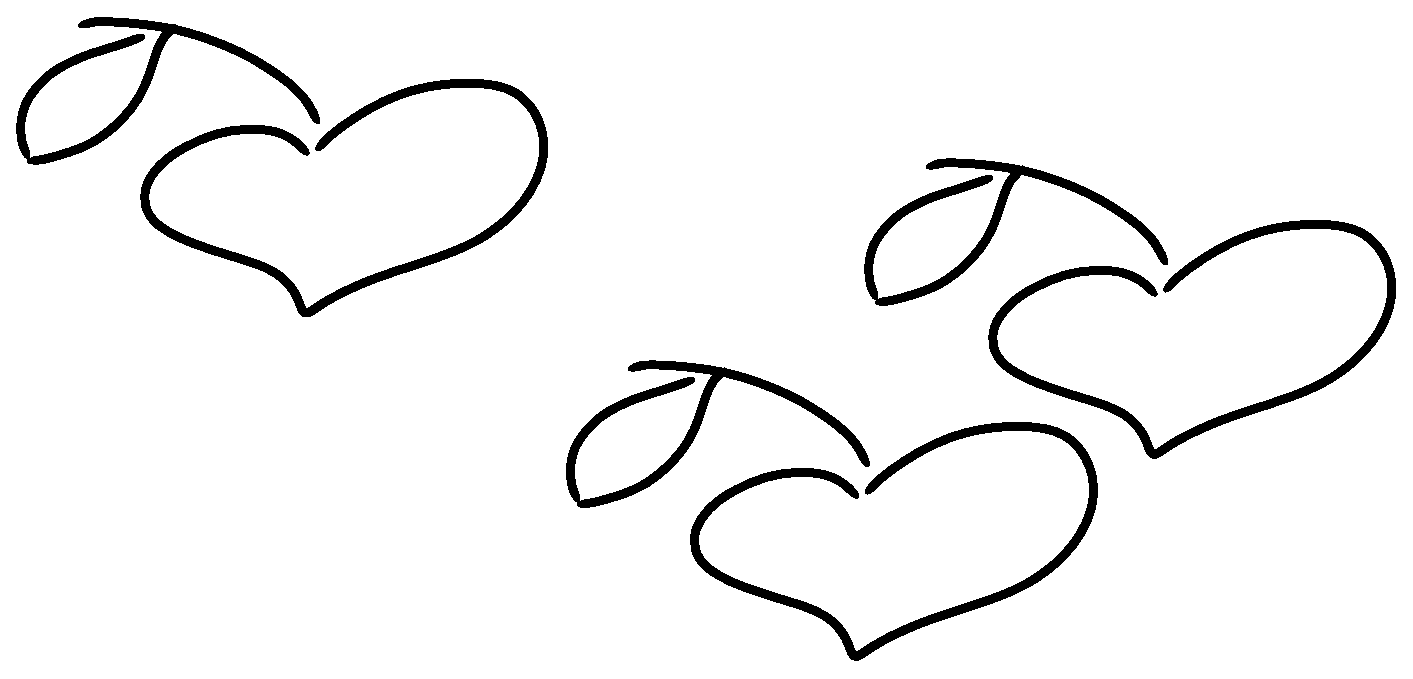
\includegraphics[width=0.6\linewidth]{images/Apples}
    %
    %\caption{
      %Одно яблоко, два яблока, ...~---~натуральные числа используются при счёте предметов.
    %}
    %\label{fig:naturals}
  %\end{figure}

  \section{Эрэн}
  
  \subsection{Предел функции (продолжение)}

  % [X] Непрерывность функции в точке
  % [X] Виды точек разрыва
  % [ ] Повторные пределы: если не равны, пределе нет? (TODO)

  Так же, как в случае~$\RR$, вводится понятие \emph{непрерывности функции в точке}.
  Функция непрерывна в точке, если значение функции в этой точке ``предсказуемо'' по её значениям в близких точках.
  Так, функция $f\colon X \hm\to \RR$, $X \hm\subset \RR^n$ называется непрерывной в точке $\bds x_0 \hm\in X$ (внутренней для~$X$), если:
  \[
    \forall \eps > 0\ \exists \delta\colon \forall \bds x\colon \rho(\bds x, \bds x_0) < \delta \to \bigl|f(\bds x) - f(\bds x_0)\bigr| < \eps
  \]

  Или, в терминах окрестностей:
  \[
    \forall \eps > 0\ \exists \delta\colon \forall \bds x \in U_{\delta}(\bds x_0) \to f(\bds x) \in U_{\delta}\bigl(f(\bds x_0)\bigr)
  \]

  Если функция~$f$ не является непрерывной в точке~$\bds x_0$, то она \emph{разрывна} в ней.
  Разрыв может быть в случаях, если~(\ref{fig:disconts}):
  \begin{itemize}
    \item функция не определена в точке (устранимый разрыв): $\not\exists f(\bds x_0)$;
    \item значение функции отличается от предела в точке (тоже устранимый разрыв): $f(\bds x_0) \hm{\not=} \lim_{\bds x \to \bds x_0} f(\bds x)$;
    \item не существует предела функции в точке (неустранимый разрыв): $\not\exists \lim_{\bds x \to \bds x_0} f(\bds x)$.
  \end{itemize}

  \begin{figure}[ht]
    \centering
    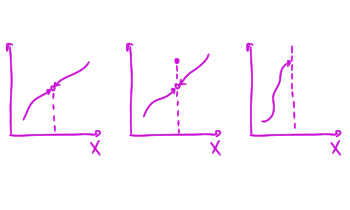
\includegraphics[width=0.6\linewidth]{images/disconts}
    
    \caption{
      Варианты разрывов функции $f\colon X \to \RR$ в точке.
      (Картинка нарисована как будто для функции одной переменной, но можно считать, что это просто такой ``упрощённый'' вариант изобразить ситуацию на $\RR^n$ (``набросок'', дающий простор для фантазии читателя).)
    }
    \label{fig:disconts}
  \end{figure}

  Кроме ``просто'' непрерывности, может рассматриваться непрерывность по какому-то множеству.
  Например, по множеству определения функции.
  Так, функция~$f$ непрерывна в~$\bds x_0$ по множеству~$X$, если:
  \[
    \forall \eps > 0\ \exists \delta\colon \forall \bds x \in U_{\delta}(\bds x_0) \textcolor{pink}{\cap X} \to f(\bds x) \in U_{\delta}\bigl(f(\bds x_0)\bigr)
  \]
  то есть смотрятся близкие точки не из всего пространства, а только из~$X$.
  По такому определению можно говорить и о непрерывности функции в \emph{изолированных} точках~$X$ (функция будет в них непрерывна).  % TODO: check? в Иванове вроде было


  \subsubsection{С3, \S 2, \textnumero 54}

  Дана функция:
  \[
    f(x, y) = \left\{
      \begin{aligned}
        &\frac{x^2 y}{x^4 + y^2},\quad & &x^2 + y^2 \not= 0\\
        &\ a,\quad & &x = y = 0
      \end{aligned}
    \right.
  \]

  Найти значение~$a$, при котором~$f(x, y)$ в точке~$(0, 0)$ будет
  \begin{itemize}
    \item непрерывной по прямой
    \[
      l\colon \left\{
        \begin{aligned}
          &x = \alpha t\\
          &y = \beta t
        \end{aligned}
      \right.,\quad \alpha^2 + \beta^2 \not= 0
    \]
    
    \item непрерывной по кривой $y \hm= \alpha x^2$

    \item ``просто'' непрерывной
  \end{itemize}
  
  \begin{solution}
    % TODO: move to theory above?
    % maybe sometime
    Что значит, что функция~$f\colon X \to \RR$ непрерывна в некоторой точке~$\bds x_0 \hm\in \RR^n$:
    \[
      \lim_{\bds x \to \bds x_0} f(\bds x) = f(\bds x_0)
    \]

    Однако в случае, если $\bds x_0$ не является внутренней точкой множества~$X$, говорить о пределе~$\lim_{\bds x \to \bds x_0}$, по-хорошему, нельзя (так как ``подходить'' к~$\bds x_0$ в данном случае не получится по произвольной ``траектории'').
    Но можно говорить о пределе \emph{по множеству определения} функции:
    \[
      \lim_{\substack{\bds x \to \bds x_0 \\ \textcolor{pink}{\bds x \in X}}} f(\bds x) = f(\bds x_0)
    \]

    А вообще, можно рассматривать пределы функций по произвольным множествам $X' \hm\subset X$:\footnote{
      Точнее, по произвольным множествам, для которых точка~$\bds x_0$ является предельной.
    }
    \[
      \lim_{\substack{\bds x \to \bds x_0 \\ \bds x \in \textcolor{pink}{X'}}} f(\bds x) = f(\bds x_0)
    \]

    Если предел функции в точке~$\bds x_0$ существует, то он будет таким же и по любому множеству.
    Но если хотя бы по какому-то множеству в точке~$\bds x_0$ нет предела (или если можно привести два множества, по которым пределы в точке существуют, но отличаются), то ``просто'' предела у функции в этой точке не будет.

    \medskip

    Итак, проверка непрерывности в точке по прямой~$l$ будет заключаться в проверке равенства:
    \[
      \lim_{\substack{(x, y) \to (0, 0) \\ (x, y) \in l}} f(x, y) \overset{?}{=} f(0, 0)
    \]

    Или, если подробнее:
    \[
      \lim_{\substack{(x, y) \to (0, 0) \\ (x, y) \in l}} \frac{x^2 y}{x^4 + y^2} \overset{?}{=} a
    \]

    Вычислим предел.
    Для этого можно выразить $x$ и $y$ через $t$ из уравнений прямой и подставить в выражение под пределом (при этом $(x, y) \hm\to (0, 0) \hm\Leftrightarrow t \hm\to 0$):
    \begin{equation*}
      \lim_{\substack{(x, y) \to (0, 0) \\ (x, y) \in l}} \frac{x^2 y}{x^4 + y^2}
        = \lim_{t \to 0} \frac{(\alpha t)^2 \beta t}{(\alpha t)^4 + (\beta t)^2}
        = \lim_{t \to 0} \frac{\alpha^2 \beta \cdot t}{\alpha^4 \cdot t^2 + \beta^2}
        = 0
    \end{equation*}
    (предел равен нулю вне зависимости от того, равен $\beta$ нулю или нет).

    Таким образом, чтобы функция была непрерывна в нуле по прямой, должно выполняться условие $a \hm= 0$.

    \medskip

    Перейдём к случаю непрерывности по кривой $y \hm= \alpha x^2$.
    Для начала можно заметить, что при $\alpha \hm= 0$ кривая становится прямой~---~этот случай уже был рассмотрен ранее (и получилось, что в этом случае должно быть $a \hm= 0$).

    Если же $\alpha \hm{\not=} 0$, то кривая $y \hm= \alpha x^2$ будет описывать параболу.

    Для проверки непрерывности по рассматриваемой кривой, можно выразить $y$ через $x$ и подставить в выражение под пределом (при этом $(x, y) \hm\to (0, 0) \hm\Leftrightarrow x \hm\to 0$):
    \[
      \lim_{\substack{(x, y) \to (0, 0) \\ y = \alpha x^2}} \frac{x^2 y}{x^4 + y^2}
        = \lim_{x \to 0} \frac{\alpha x^4}{x^4 + \alpha^2 x^4} = \frac{\alpha}{1 + \alpha^2}
    \]

    Таким образом, непрерывность в нуле по параболе $y \hm= \alpha x^2$ будет при условии:
    \[
      a = \frac{\alpha}{1 + \alpha^2}
    \]

    Также можно заметить, что для разных парабол, скажем, для $y \hm= x^2$ и $y \hm= -x^2$, значения~$a$, дающие непрерывность, будут разными.

    \medskip

    Из сказанного получаем, что ``просто'' непрерывной в нуле функция ни при каких~$a$ не будет (разные $a$ для прямых и парабол, разные $a$ для разных парабол~---~для разных множеств условия непрерывности отличаются).
    
  \end{solution}

  
  \subsubsection{С3, \S 2, \textnumero 62(5)}

  Найти все точки разрыва (устранимого и нет) функции двух переменных:
  \[
    f(x, y) = \left\{
      \begin{aligned}
        &\frac{x^3 + y^3}{x + y}, & &\mbox{если}\ x + y \not= 0\\
        &\ 3,                     & &\mbox{если}\ x + y = 0
      \end{aligned}
    \right.
  \]
  
  \begin{solution}
    В каждой точке $(x_0, y_0)$ не на прямой $l\colon x \hm+ y \hm= 0$ функция задаётся ``нормальной'' (не кусочной) формулой (в каждой точке, а также в некоторой её окрестности).
    Формулой, которая, очевидно, задаёт непрерывную функцию:
    \[
      f(x, y) = \frac{x^3 + y^3}{x + y} = x^2 - xy + y^2,\quad x + y \not= 0
    \]

    Вопросы возникают только по поводу точек прямой~$l$.

    Пусть $(x_0, y_0) \hm\in l$.
    Будем проверять непрерывность в точке по определению:
    \[
      \lim_{(x, y) \to (x_0, y_0)} f(x, y) \overset{?}{=} f(x_0, y_0)
    \]

    Очевидно, если считать предел в точке прямой~$l$ по самой прямой~$l$, то непрерывность будет:
    \[
      \lim_{\substack{(x, y) \to (x_0, y_0) \\ (x, y) \in l}} f(x, y) = 3 = f(x_0, y_0)
    \]

    Посмотрим на ``просто'' предел:\footnote{
      На самом деле это тоже не ``просто'' предел~---~тоже предполагаем, что сходимся к точке по множеству~---~по множеству, не включающему в себя точки прямой~$l$ (ведь только для них работает формула, которая стоит под пределом).
      Если же всё-таки посмотреть на предел в целом, без ограничения по множеству, то что может получиться: при $x \hm\to x_0$ встречаются как точки на прямой~$l$, так и вне её.
      С точками на прямой уже показали, что по ним~$f(\bds x)$ сходится к~$3$.
      Чтобы предел существовал,~$3$ должна в пределе получаться и для значений функции на точках вне прямой.
    }
    \begin{equation*}
    \begin{split}
      \lim_{(x, y) \to (x_0, y_0)} f(x, y) &= \lim_{(x, y) \to (x_0, y_0)} x^2 - xy + y^2
      = x_0^2 - x_0 y_0 + y_0^2 \xrightarrow{x_0 + y_0 = 0} 3 x_0^2 \overset{\?}{=} 3
    \end{split}
    \end{equation*}

    Видно условие непрерывности в точке на прямой: $x_0^2 \hm= 1 \hm\leftrightarrow x_0 \hm= \pm 1$.
    Только в точках прямой с такими $x$-координатами функция~$f$ будет непрерывна.
    Эти точки: $(\pm 1, \mp 1)$.
    В остальных точках прямой~$l$ функция терпит устранимый разрыв (предел есть, но не равен значению функции в точке).
  \end{solution}



  \subsection{Производные. Дифференциал}

  % [X] Дифференциал функции одной переменной (взять из того семестра с картинкой)
  % [X] Частные производные (+ картинка)
  % [X] Дифференциал, дифференцируемость !<=> существование всех частных производных (как пункт в номере)
  % [X] Производная по направлению

  \subsubsection{Производная и дифференциал на прямой (вспоминание)}  % Some error in XeTeX: на~$\RR$ (вспоминание)

  Вспомним производную и дифференциал, какие они были для числовых функций.

  Производная функции~$f\colon \RR \hm\to \RR$ показывает ``скорость'' её изменения в точке~$x_0$:
  \begin{equation}\label{eq:derivative-in-R}
  \begin{split}
    \frac{\diff f}{\diff x} \equiv f'(x_0)
      &= \lim_{x \to x_0} \frac{f(x) - f(x_0)}{x - x_0}\\
      &= \lim_{\Delta x \to 0} \frac{f(x_0 + \Delta x) - f(x_0)}{\Delta x}
  \end{split}
  \end{equation}
  Производная несёт информацию, с одной стороны, о том, как быстро меняется функция (модуль производной), но также рассказывает о ``характере'' изменения: увеличивается функция при проходе через~$x_0$ или, наоборот, уменьшается (знак производной).

  Геометрический смысл производной~---~тангенс угла наклона касательной к графику функции $y \hm= f(x)$ в точке~$x_0$ (касательная~---~как предел секущей при $x \hm\to x_0$).

  \begin{figure}[ht]
    \centering
      
    \includegraphics[width=0.6\linewidth]{images/diff-f-df}
      
    \caption{Вблизи точки~$x_0$ значение функции $f(x) \hm\approx f(x_0) \hm+ f'(x_0) \cdot (x - x_0)$.}
    \label{fig:diff-f}
  \end{figure}

  Вообще же, в ``близкой'' окрестности точки $x_0$ график функции ``в некотором приближении'' представим как раз как график касательной в точке~$x_0$~(\ref{fig:diff-f}),\footnote{
    Источник: \href{https://github.com/Alvant/Mathematichalys/tree/master}{МА-1, семинар про дифференциал (шестой)}.
    % TODO: вставить более точную ссылку после рефактора структуры репозитория
  }~---~чем ближе окрестность, тем точнее такое представление~---~то есть приращение $\Delta f(x_0) \hm= f(x) \hm- f(x_0)$ в точке~$x_0$ функции можно ``оценить'' так:
  \[
    f(x) - f(x_0) \approx f'(x_0) \cdot (x - x_0)
  \]

  Оказывается, что можно написать и ``нормальное'' (строгое) равенство без приближений:
  \[
    f(x) - f(x_0) = f'(x_0) \cdot (x - x_0) + o(x - x_0),\quad x \to x_0
  \]
  где $o(x - x_0)$ есть $o$-малая от $x \hm- x_0$, то есть некоторая функция $g(x)$, для которой верно, что $\lim_{x \to x_0} \frac{g(x)}{x - x_0} \hm= 0$.
  (Поправка, отвечающая за ``точность'' приближения приращения функции как линейной функции от приращения аргумента~---~чем ближе к~$x_0$, тем точнее.)
  % (Таким образом, строчка выше~---~не совсем равенство в привычном смысле, это как бы ``равенство в пределе''.)
  Итого, для значения~$f(x)$ функции в некоторой точке~$x$ можно записать:
  \[
    f(x) = f(x_0) + f'(x_0) \cdot (x - x_0) + o(x - x_0),\quad x \to x_0
  \]

  Из этого соотношения возникают два понятия.
  
  \emph{Дифференциалом независимой переменной} называется её приращение:
  \[
    \diff x = \Delta x = x - x_0
  \]

  \emph{Дифференциалом функции} в точке~$x_0$ называется линейная по $\diff x$ часть приращения функции в этой точке (линейное ``приближение'' приращения функции):
  \begin{equation}\label{eq:diff-f}
    \diff f(x_0) = f'(x_0) \diff x   % f'(x_0) (x - x_0) = 
  \end{equation}

  % Тогда значение функции в точке~$x$ можно записать с помощью дифференциалов:
  % \[
  %   f(x) = f(x_0) + \underbrace{f'(x_0) \diff x}_{\diff f(x_0)} + o(x - x_0),\quad x \to x_0
  % \]

  А \emph{дифференцированием} называется процесс взятия производной функции.
  При этом получение дифференциала~\eqref{eq:diff-f} по сути тоже сводится к взятию производной.
  И правила дифференцирования функций во многом повторяют соответствующие правила для производных.
  Например, дифференциал константы $c \hm\in \RR$ равен нулю $\diff c \hm= 0$.
  Дифференциал суммы равен сумме дифференциалов.
  Константу как множитель можно выносить за знак дифференциала.
  
  Дифференциал произведения (распишем его подробнее):
  \[
    \diff (fg) = \diff f \cdot g + f \cdot \diff g
  \]
  так как, с одной стороны:
  \[
    \diff (fg) = (fg)' \diff x = (f'g + fg') \diff x
  \]
  и, с другой стороны:
  \[
    \diff f \cdot g + f \cdot \diff g = f' \diff x \cdot g + f \cdot g' \diff x
      = (f' g + fg') \diff x
  \]

  Дифференциал частного:
  \[
    \diff \left(\frac{f}{g}\right) = \frac{\diff f \cdot g - f \cdot \diff g}{g^2}
  \]


  \subsubsection{Производная и дифференциал в многомерии}  % Some error in XeTeX: в~$\RR^n$}

  В многомерном пространстве формула~\eqref{eq:derivative-in-R} не применима и обобщить её не очень понятно, как: ведь теперь ``движение'' от $\bds x$ к $\bds x_0$ происходит в~$\RR^n$, и разность $\bds x \hm- \bds x_0$ будет вектором.
  Можно бы было посчитать \emph{длину} этого вектора и поставить в знаменателе~\eqref{eq:derivative-in-R}~---~но тогда это уже была бы не производная, потому что потерялась бы информация о направлении движения от $\bds x$ к $\bds x_0$ ($|\bds x \hm- \bds x_0|$~---~это лишь часть информации об изменении аргумента).

  То есть основная ``проблема'' в том, что переменных теперь много, они все могут меняться.

  Поэтому можно (немного ``искусственно'') упростить картину так, чтобы всё-таки можно было ввести производную аналогично~\eqref{eq:derivative-in-R} (и при этом ввести её так, чтобы она обобщала производную в~$\RR$).
  \emph{Будем следить за изменением функции не сразу по всем переменным, а только по одной.}

  Рассмотрим для наглядности функцию на плоскости: $f(x, y)$, где $(x, y)$~---~это компоненты двумерного вектора: $\bds x \hm= (x, y)$.
  Пусть есть точка $(x_0, y_0)$.
  \emph{Зафиксируем} координату $y_0$, тогда разность $f(x, \textcolor{grey}{y_0}) \hm- f(x_0, \textcolor{grey}{y_0})$ будет показывать изменение функции только при изменении~$x$.
  Получается так, словно $f$~---~это теперь функция одной переменной~$x$ (на самом деле функция многих переменных, просто при зафиксированных всех, кроме одной), поэтому можно посчитать её производную так же, как в~$\RR$.
  Таким образом посчитанная производная называется \emph{частной производной} функции $f(x, y)$ по~$x$:
  \begin{equation*}
  \begin{split}
    \frac{\partial f}{\partial x} \equiv f'_x
      &= \lim_{x \to x_0} \frac{f(x, \textcolor{grey}{y_0}) - f(x_0, \textcolor{grey}{y_0})}{x - x_0}\\
      &= \lim_{\Delta x \to 0} \frac{f(x_0 + \Delta x, \textcolor{grey}{y_0}) - f(x_0, \textcolor{grey}{y_0})}{\Delta x}
  \end{split}
  \end{equation*}

  Аналогичным образом рассчитываются частные производные и по другим переменным (в данном случае~---~только по~$y$):
  \begin{equation*}
  \begin{split}
    \frac{\partial f}{\partial y} \equiv f'_y
      &= \lim_{y \to y_0} \frac{f(\textcolor{grey}{x_0}, y) - f(\textcolor{grey}{x_0}, y_0)}{y - y_0}\\
      &= \lim_{\Delta y \to 0} \frac{f(\textcolor{grey}{x_0}, y_0 + \Delta y) - f(\textcolor{grey}{x_0}, y_0)}{\Delta y}
  \end{split}
  \end{equation*}

  Частные производные не дают полной информации о ``динамике'' изменения функции при $x \hm\to x_0$, но они показывают скорость изменения функции в $x_0$ вдоль соответствующих осей.

  Функция в $\RR^2$ называется \emph{дифференцируемой} в точке~$(x_0, y_0)$, если в её окрестности верна формула:
  \begin{equation}\label{eq:base-diff-in-Rn}
    f(x, y) = f(x_0, y_0) + A \Delta x + B \Delta y + o(\rho),\ \rho \to 0,\quad \rho \equiv \sqrt{(x - x_0)^2 + (y - y_0)^2}
  \end{equation}
  где $A, B \in \RR$, а $\Delta x \hm= x \hm- x_0$ и $\Delta y \hm= y \hm- y_0$.
  То есть если приращение функции линейно зависит от приращений аргументов при $\rho \hm\to 0$.

  И \emph{если} функция дифференцируема, то:
  \begin{equation}\label{eq:diff-in-Rn}
    f(x, y) = f(x_0, y_0) + \underbrace{\frac{\partial f}{\partial x} (x_0, y_0) \Delta x + \frac{\partial f}{\partial y} (x_0, y_0) \Delta y}_{\diff f(x_0, y_0)} + o(\rho),\ \rho \to 0
  \end{equation}
  где $\diff f(x_0, y_0)$~---~дифференциал функции в точке (линейное приближение её приращения в точке).
  % Линейное приближение приращения функции в точке называется её дифференциалом:
  % \[
  %   \diff f(x_0, y_0) = \frac{\partial f}{\partial x} (x_0, y_0) \diff x + \frac{\partial f}{\partial y} (x_0, y_0) \diff y
  % \]
  % где $\diff x \hm\equiv \Delta x \hm= x \hm- x_0$ и $\diff y \hm\equiv \Delta y \hm= y \hm- y_0$.
  (Но в $\RR^n$ из того, что у функции в точке есть частные производные, вообще ещё не следует, что она дифференцируема~---~подробнее см. номер~(\ref{sec:s3-par3-12}).

  Кроме ``просто'' дифференциала, можно рассмотреть дифференциалы по отдельным переменным (при всех остальных фиксированных).
  Так, например, при константной $y \hm\equiv y_0$ будет:
  \[
    \diff_x f(x_0, y_0) \equiv \diff f(x_0, y_0)|_{y = y_0} = \frac{\partial f}{\partial x}(x_0, y_0) \diff x
  \]

  И в таком случае можно выразить частную производную через \emph{отношение дифференциалов}:
  \[
    \frac{\partial f}{\partial x} = \frac{\diff_x f}{\diff x}
  \]

  А дифференциал функции в точке можно записать в виде суммы дифференциалов по отдельным переменным:
  \[
    \diff f = \diff_x f + \diff_y f
  \]

  Кроме частных производных, для функций в~$\RR^n$ рассматриваются \emph{производные по направлению}.
  Производная по направлению рассчитывается при ``движении'' к точке вдоль проходящей через неё прямой, которая задаётся вектором~$\bds a \hm\in \RR^n$~(\ref{fig:der-on-vec}).
  % вдоль исходящего из неё луча, направление которого задаётся вектором в~$\RR^n$.
  В отличие от частных производных (где ``движение'' к точке происходит вдоль оси), изменение функции будет определяться изменением \emph{сразу по нескольким} переменным.
  Что тогда поставить в знаменателе дроби (предел которой будет производной)?
  При движении по прямой к точке в качестве изменения аргумента можно считать просто \emph{расстояние} от текущей точки $\bds x$ до ``нулевой'' $\bds x_0$~---~причём расстояние со знаком: с ``плюсом'', если точка $\bds x$ получается из $\bds x_0$ движением в направлении вектора~$\bds a$ (то есть
  % $(\bds x \hm- \bds x_0) \hm\upuparrows \bds a$),
  $(\bds x \hm- \bds x_0) \hm{\upups} \bds a$),
  и с ``минусом'', если точка $\bds x$ лежит с другой стороны от $\bds x_0$ (то есть $(\bds x \hm- \bds x_0) \hm{\updowns} \bds a$).
  % upuparrows use heads like in "old-arrows" (The Comprehensive LaTeX Symbol List -- https://mirror.truenetwork.ru/CTAN/info/symbols/comprehensive/symbols-a4.pdf)
  % so remove upuparrows to make look more like custom updownarrows
  \footnote{
    Существует и \href{https://en.wikipedia.org/wiki/Directional_derivative\#Definition}{другой подход к расчёту производной вдоль вектора}: когда единичный ``шаг'' полагается равным длине вектора (шагаем к точке $\bds x_0$ вдоль вектора с шагом длиной в вектор).
  }

  \begin{figure}[ht]
    \centering
    \includegraphics[width=0.5\linewidth]{images/der-on-vec}
    
    \caption{
      К производной по направлению в точке~$(x_0, y_0)$ вдоль вектора~$\bds a$.
    }
    \label{fig:der-on-vec}
  \end{figure}

  Итак, распишем на примере~$\RR^2$ производную функции $f(x, y)$ вдоль вектора~$\bds a \hm= (a_x, a_y)$:
  \[
    \frac{\partial f}{\partial \bds a}(x_0, y_0) = \lim_{t \to 0} \frac{f(x_0 + t a_x, y_0 + t a_y) - f(x_0, y_0)}{t |\bds a|}
  \]

  Если вектор $\bds a$ единичный ($|\bds a| \hm= 1$), то производная вдоль него:
  \begin{equation}\label{eq:derivative-along-vector}
    \frac{\partial f}{\partial \bds a}(x_0, y_0) = \lim_{t \to 0} \frac{f(x_0 + t a_x, y_0 + t a_y) - f(x_0, y_0)}{t}
  \end{equation}

  Таким образом, производная по направлению~---~это не что-то ``другое совсем новое''~---~она обобщает понятие частной производной: частные производные~---~это производные вдоль направлений осей координат.
  

  \subsubsection{С3, \S 3, \textnumero 3(6)}

  Найти частные производные первого порядка функции:
  \[
    f(x, y, z) = \left(\frac{x}{y}\right)^{\! z}  % TODO: why we need \! here? I mean, why things look worse without it?
  \]
  
  \begin{solution}
    Частные производные~---~производные по одной переменной.
    Чтобы их найти, можно просто дифференцировать по нужной переменной формулу, которой задаётся функция, считая все остальные переменные как бы постоянными (константами):
    \[
      % https://tex.stackexchange.com/questions/40124/how-to-reduce-hspace-between-columns-in-align-environment
      % https://www.latex-project.org/help/documentation/amsldoc.pdf
      % \left\{
        \begin{alignedat}{3}
          &\frac{\partial f}{\partial x} & \quad &= \quad z \left(\frac{x}{y}\right)^{\! z - 1} \cdot \frac{1}{y} & \quad  &= \quad \frac{z}{x} f(x, y, z)\\
          &\frac{\partial f}{\partial y} & &= \quad z \left(\frac{x}{y}\right)^{\! z - 1} \cdot \left(-\frac{x}{y^2}\right) & &= \quad -\frac{z}{y} f(x, y, z)\\
          &\frac{\partial f}{\partial z} & &= \quad \left(\exp\left\{z \cdot \ln\frac{x}{y}\right\}\right)' & &= \quad f(x, y, z) \ln \frac{x}{y}
        \end{alignedat}
      % \right.
    \]
  \end{solution}
  

  \subsubsection{С3, \S 3, \textnumero 12}\label{sec:s3-par3-12}

  Верны ли для функции~$f(x)$, $x \hm\in \RR^n$ следующие утверждения?

  \begin{todolist}
      % Верно при n = 1
      \item[\halffailed] Если функция в некоторой точке имеет частные производные по всем переменным, то она непрерывна в этой точке.

      % Верно при n = 1
      \item[\halffailed] Если функция в каждой точке пространства~$\RR^n$ имеет частные производные по всем переменным, то она непрерывна в~$\RR^n$.
      
      \item[\done] Если функция дифференцируема в некотором точке, то в этой точке у функции существуют частные производные по всем переменным.

      % Верно при n = 1
      \item[\halffailed] Если у функции в некоторой точке существуют частные производные по всем переменным, то она дифференцируема в этой точке.
      
      \item[\failed] Если функция дифференцируема в некотором точке, то в этой точке у функции существуют \emph{непрерывные} частные производные по всем переменным.

      \item[\done] Если у функции в некоторой точке существуют \emph{непрерывные} частные производные по всем переменным, то она дифференцируема в этой точке.
    \end{todolist}
  
  \begin{solution}
    \mbox{}\par
    
    \textcolor{yellow}{
      \emph{Если функция в некоторой точке имеет частные производные по всем переменным, то она непрерывна в этой точке?
    }}

    В случае функции одной переменной~---~это правда, потому что частная производная для неё~---~это такая производная, которая строится по оценке ``общего'' изменения функции в окрестности точки.
    Непрерывность~---~тоже про про поведение функции вблизи точки ``в целом''.
    \[
      \exists \lim_{x \to x_0} \frac{f(x) - f(x_0)}{x - x_0} \quad\Rightarrow\quad \lim_{x \to x_0} f(x) = f(x_0)
    \]

    Но для функций в пространстве~$\RR^n$, $n \hm\geq 2$ утверждение вообще перестаёт работать.
    Потому что теперь частные производные~---~характеризующие изменения функции только вдоль соответствующих осей~---~не говорят о поведении функции в окрестности точки ``в целом'' (если про функцию ничего дополнительно не требовать).

    Для большей конкретики рассмотрим пример функции в пространстве~$\RR^2$:
    \begin{equation}\label{eq:example-partial-not-diff}
      f(x, y) = \left\{
        \begin{alignedat}{2}
          &\frac{xy}{x^2 + y^2},\quad & &x^2 + y^2 \not= 0\\
          &\ 0, \quad & &x = y = 0
        \end{alignedat}
      \right.
    \end{equation}

    Очевидно, у этой функции ``интересная'' точка~---~это $(0, 0) \hm\equiv (x_0, y_0)$ (в остальных точках точно всё ``хорошо'').
    Поэтому проверим для неё: наличие частных производных и непрерывность.

    Частные производные (считаем по определению):
    \[
      \begin{alignedat}{3}
      &\frac{\partial f}{\partial x}(x_0, y_0) & \quad &= \lim_{\Delta x \to 0} \frac{f(x_0 + \Delta x, \textcolor{grey}{y_0}) - f(x_0, \textcolor{grey}{y_0})}{\Delta x} = \lim_{\Delta x \to 0} \frac{0 - 0}{\Delta x} & \quad &= \quad 0\\
      &\frac{\partial f}{\partial y}(x_0, y_0) & &=  / \mbox{аналогично} / & &= \quad 0
      \end{alignedat}
    \]

    Но непрерывна ли данная функция в нуле?
    \[
      \lim_{(x, y) \to (x_0, y_0)} f(x, y) \overset{\?}{=} f(x_0, y_0)
    \]

    Если предел в нуле существует, то можно попробовать его посчитать по некоторым ``удобным'' множествам...
    \[
      \lim_{(x, y) \to (0, 0)} \frac{xy}{x^2 + y^2} = \left\{
        \begin{alignedat}{3}
          &\lim_{\substack{x \to 0 \\ y = x}} & &\frac{x^2}{2x^2} & &= \hphantom{+}\frac{1}{2}\\
          &\lim_{\substack{x \to 0 \\ y = -x}} & &\frac{-x^2}{2x^2} & &= -\frac{1}{2}\\
          &\lim_{\substack{x \to 0 \\ y = 0}} & &\frac{0}{x^2} & &= \hphantom{+}0\\
          &\ldots
        \end{alignedat}
      \right.
    \]

    Уже по двум прямым $y \hm= \pm x$ предел в точке~$(0, 0)$ получился разным.
    Значит, ``просто'' предела в точке у функции нет.
    (Если бы он был, он был бы таким же по любому множеству, ``касающемуся'' точки.)

    \medskip

    \textcolor{yellow}{
      \emph{Если функция в каждой точке пространства~$\RR^n$ имеет частные производные по всем переменным, то она непрерывна в~$\RR^n$?
    }}

    В случае функции на~$\RR$ утверждение снова верное.

    С функцией на~$\RR^n$, вообще говоря, можно бы было и задуматься (не является ли требование наличия частных производных \emph{во всех} точках настолько сильным: ведь если в данной точке есть частные производные и во всех точках сколь угодно близко к ней~---~тоже, то нельзя ли отсюда сделать положительный вывод о непрерывности?..)

    Однако пример из прошлого пункта~\eqref{eq:example-partial-not-diff} показывает, что в~$\RR^n$ сказанное в общем случае тоже не верно.

    \medskip

    \textcolor{green}{
      \emph{Если функция дифференцируема в некотором точке, то в этой точке у функции существуют частные производные по всем переменным?
    }}

    Очевидно, пункт снова верен для функций на~$\RR$: дифференцируемость для них равносильна существованию производной:
    \begin{equation*}
    \begin{split}
      f(x) = f(x_0) + A \Delta x + o(\Delta x),\  \Delta x \to 0
      \quad \Leftrightarrow\quad
      \exists \frac{\diff f}{\diff x}(x_0) = A
    \end{split}
    \end{equation*}

    Потому что:
    \begin{equation*}
    \begin{split}
      A &= f'(x_0) = \lim_{x \to x_0} \frac{f(x) - f(x_0)}{\Delta x} \in \RR\\
      &\Leftrightarrow \lim_{x \to x_0} \frac{f(x) - f(x_0)}{\Delta x} - A = 0\\
      &\Leftrightarrow \lim_{x \to x_0} \frac{f(x) - f(x_0) - A \Delta x}{\Delta x} = 0
      \Leftrightarrow f(x) - f(x_0) - A \Delta x = o(\Delta x),\ \Delta x \to 0
    \end{split}
    \end{equation*}

    Оказывается, что утверждение остаётся верным и для функций на~$\RR^n$!
    Попытаться объяснить это ``на пальцах'' можно следующим образом.
    Дифференцируемость~---~это комплексное понятие, описывающее возможность линейного приближения функции в окрестности точки; дифференцируемость~---~про то, что можно ``предсказать'' значение~$f(\bds x)$ по значению~$f(\bds x_0)$ и разницам (покоординатным) между $\bds x$ и~$\bds x_0$.
    % (зная ``скорости изменения'' функции по каждой координате).
    Таким образом, в определении дифференцируемости уже как бы лежит возможность оценки общего изменения функции по её ``отдельным'' изменениям вдоль каждой из осей.
    %~---~по частным производным.

    Покажем на примере функции на~$\RR^2$, что существование частных производных следует из дифференцируемости так же, как и в~$\RR$.
    Функция $f(x, y)$ дифференцируема в точке~$(x_0, y_0)$, если:
    \[
      \Delta f(x_0, y_0) = A \Delta x + B \Delta y + o(\rho),\ \rho \to 0,\quad \rho \equiv \sqrt{(x - x_0)^2 + (y - y_0)^2}
    \]

    Но тогда, например, при $y \hm\equiv y_0 \hm= \mathrm{const}$ будет:
    \[
      \Delta_x f(x_0, y_0) = A \Delta x + 0 + o(\Delta x),\ \Delta x \to 0
    \]
    где в качестве $\Delta_x f$ обозначено приращение функции при условии, что все переменные (в данном случае всего одна), кроме~$x$, считаются константными и равными соответствующим ``нулевым'' значениям.
    Отсюда и из рассмотренного ранее случая~$\RR$ сразу видно, что:
    \[
      A = \lim_{\Delta x \to 0} \frac{\Delta_x f}{\Delta x} (x_0, y_0) = \frac{\diff_x f}{\diff x} (x_0, y_0) = \frac{\partial f}{\partial x}(x_0, y_0)
    \]
    где как $\diff_x f$ обозначен дифференциал функции по переменной~$x$.
    
    Аналогично с частной производной по~$y$ в точке.

    \medskip
    
    \textcolor{yellow}{
      \emph{Если у функции в некоторой точке существуют частные производные по всем переменным, то она дифференцируема в этой точке?
    }}

    В случае~$\RR$ дифференцируемость равносильна наличию конечной производной, поэтому данное утверждение в~$\RR$ также выполняется.

    Но покажем на примере, что в~$\RR^n$ ($n \hm\geq 2$) из существования всех частных производных (скоростей изменения функции вдоль осей) дифференцируемость (``предсказуемость'' изменения функции в окрестности) вообще не следует.

    Вспомним~\eqref{eq:example-partial-not-diff} такую функцию на плоскости~(\ref{fig:paper-list}):
    \[
      f(x, y) = \left\{
        \begin{alignedat}{2}
          &\frac{xy}{x^2 + y^2},\quad & &x^2 + y^2 \not= 0\\
          &\ 0, \quad & &x = y = 0
        \end{alignedat}
      \right.
    \]

    \begin{figure}[ht]
      \centering
      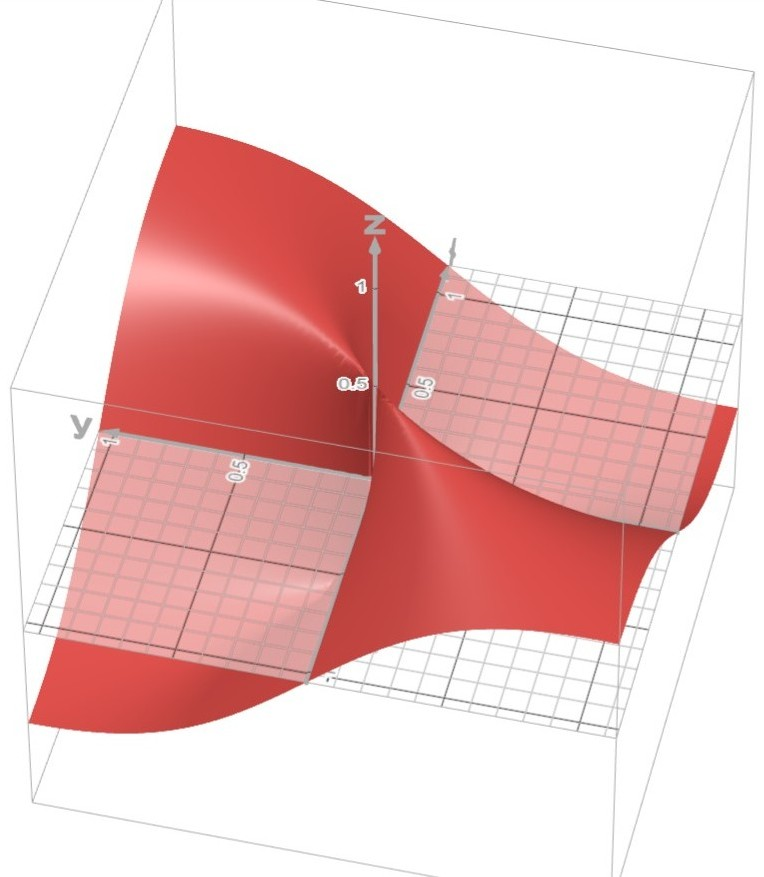
\includegraphics[width=0.4\linewidth]{images/paper-list-cut}
    
      \caption{
        \href{https://www.desmos.com/3d}{График} функции~\eqref{eq:example-partial-not-diff}, у которой есть частные производные в нуле, но которая не дифференцируема в нуле.
        (Похож на лист бумаги, согнутый так, что ровно по осям он на нуле, а в других местах (особенно по ``диагоналям'') изогнут сильно~---~то есть глядя только на оси нельзя ничего сказать об изменении в районе нуля в целом.
        Отметим также, что если ``повернуть'' график, рассмотрев таким образом, например, функцию ${f(x, y) \hm= \frac{(x - y)(x + y)}{(x - y)^2 + (x + y)^2}}$, то у неё в нуле не будет даже частных производных.)
      }
      \label{fig:paper-list}
    \end{figure}

    В сюжете про непрерывность (её отсутствие) у этой функции в нуле уже показали, что частные производные в нуле существуют и равны нулю.
    Проверим теперь дифференцируемость (её отсутствие) в нуле.

    Если функция дифференцируема в нуле $(0, 0) \hm\equiv (x_0, y_0)$, то можно записать:
    \[
      f(x, y) = f(x_0, y_0) + \frac{\partial f}{\partial x}(x_0, y_0) \Delta x + \frac{\partial f}{\partial y}(x_0, y_0) \Delta y + o(\rho),\ \rho \to 0,\quad \rho \equiv \sqrt{(x - x_0)^2 + (y - y_0)^2}
    \]

    Подставляя значение функции и частных производных в нуле, получаем:
    \[
      \frac{xy}{x^2 + y^2} = 0 + 0 + 0 + o(\rho) = o(\rho),\ \rho \to 0
    \]

    Верно ли это равенство?
    Иными словами, надо проверить, верно ли, что:
    \[
      \lim_{\rho \to 0} \left(\frac{xy}{x^2 + y^2} \Big/ \rho\right) = 0 \quad \Leftrightarrow \quad \lim_{(x, y) \to (0, 0)} \frac{xy}{(x^2 + y^2)^{3/2}} = 0
    \]

    (Сверху стоит что-то квадратичное относительно $x$ и $y$, степень же снизу $2 \hm\cdot 3 \hm/ 2 \hm= 3$, поэтому сомнительно, чтобы в пределе получился ноль, ведь в пределе одной переменной $x^2 \hm/ x^3$ при $x \to 0$ нуля не будет.)

    Рассмотрим этот предел по множеству $y \hm= x$:
    \[
      \lim_{\substack{(x, y) \to (0, 0) \\ y = x}} \frac{xy}{(x^2 + y^2)^{3/2}} = \lim_{x \to 0} \frac{x^2}{2^{3/2} x^3} = \infty \not= 0
    \]

    Значит, ``просто'' предел, без указания конкретного множества сходимости~---~это точно не ноль.

    \medskip
    
    \textcolor{red}{\emph{
      Если функция дифференцируема в некоторой точке, то в этой точке у функции существуют \emph{непрерывные} частные производные по всем переменным?
    }}

    (Сразу не очень понятно, почему частные производные вдруг должны ещё оказаться непрерывными, то есть утверждение заранее вызывает сомнения...)

    Рассмотрим пример функции на~$\RR^2$:
    \begin{equation}\label{eq:example-diff-not-cont-partial}
        f(x, y) = \left\{
          \begin{alignedat}{2}
            &(x^2 + y^2) \sin\left(\frac{1}{\sqrt{x^2 + y^2}}\right),\quad & &x^2 + y^2 \not= 0\\
            &\ 0,\quad & &x = y = 0
          \end{alignedat}
        \right.
    \end{equation}

    Проверим, что функция дифференцируема (в нуле~---~из формулы~\eqref{eq:example-diff-not-cont-partial} видно, что интерес будет представлять эта точка), но что хотя бы одна частная производная (а раз одна, то и другая, потому что формула~\eqref{eq:example-diff-not-cont-partial} симметрична относительно переменных $x$ и $y$) не будет непрерывной в нуле.

    Частные производные:
    \[
      \begin{alignedat}{3}
        &\frac{\partial f}{\partial x}(0, 0) & \quad &= \lim_{\Delta x \to 0} \frac{f(0 + \Delta x, \textcolor{grey}{0}) - f(0, \textcolor{grey}{0})}{\Delta x} = \lim_{\Delta x \to 0} \frac{\Delta x^2 \sin\left(\frac{1}{|\Delta x|}\right)}{\Delta x} & \quad &= \quad 0\\
        &\frac{\partial f}{\partial y}(0, 0) & &=  / \mbox{аналогично} / & &= \quad 0
      \end{alignedat}
    \]

    Дифференцируемость (проверяем отдельно):
    \[
      f(x, y) \overset{\?}{=} f(x_0, y_0) + \frac{\partial f}{\partial x}(x_0, y_0) \Delta x + \frac{\partial f}{\partial y}(x_0, y_0) \Delta y + o(\rho),\ \rho \to 0,\quad \rho \equiv \sqrt{(x - x_0)^2 + (y - y_0)^2}
    \]
    \[
      f(x, y) = 0 + 0 + 0 + o(\rho),\ \rho \to 0
    \]
    \[
      \lim_{(x, y) \to (0, 0)} \frac{f(x, y)}{\rho} = \lim_{(x, y) \to (0, 0)} \sqrt{x^2 + y^2} \sin\left(\frac{1}{\sqrt{x^2 + y^2}}\right) = 0
    \]
    так как $(x, y) \hm\to (0, 0) \hm\Leftrightarrow \sqrt{x^2 + y^2} \hm\to 0$.

    И наконец~---~проверим непрерывность частной производной (например, по~$y$) в нуле:
    \[
      \lim_{(x, y) \to (x_0, y_0)} \frac{\partial f}{\partial y} (x, y) \overset{\?}{=} \frac{\partial f}{\partial y} (x_0, y_0)
    \]

    Находим частную производную по~$y$ в точке просто по формуле функции~\eqref{eq:example-diff-not-cont-partial} (ведь $(x, y) \hm{\not=} (0, 0)$) и подставляем под предел:
    \[
      \lim_{(x, y) \to (x_0, y_0)} \frac{\partial f}{\partial y} (x, y) = \lim_{(x, y) \to (0, 0)} \left\{2y \cdot \sin\left(\frac{1}{\sqrt{x^2 + y^2}}\right) - \frac{y}{\sqrt{x^2 + y^2}} \cdot \cos\left(\frac{1}{\sqrt{x^2 + y^2}}\right) \right\} = 0 + \pumpkin
      % (x^2 + y^2) \cdot \cos\left(\frac{1}{\sqrt{x^2 + y^2}}\right) \cdot \left(-\frac{1}{2 (x^2 + y^2)^{3/2}}\right) \cdot 2y \right\}
    \]
    первое слагаемое под пределом стремится к нулю, второе же ни к чему не стремится, потому что имеет вид $\cos \phi (x, y) \hm\cdot \cos\left(\frac{1}{\sqrt{x^2 + y^2}}\right)$~---~то есть ограничено, но при $(x, y) \hm\to (0, 0)$ может ``скакать'' туда-сюда (чтобы было не так ``рокомахательно'', можно, к примеру, рассмотреть предел от второго слагаемого по прямой $y \hm= x$~--~или даже лучше по прямой $x \hm= 0$).
    % ~---~или даже лучше взять пределы по лучу $y \hm= x \hm> 0$ и $y \hm= x \hm< 0$).

    Таким образом, частные производные не являются непрерывными в нуле.

    На самом деле... можно бы было придумать пример и для случая~$\RR$)

    Возьмём ``аналог'' рассмотренной только что функции, только теперь на прямой:
    \[
      f(x) = \left\{
        \begin{aligned}
          &x^2 \sin\frac{1}{x}, & &x \not= 0\\
          &0, & &x = 0
        \end{aligned}
      \right.
    \]

    Читателю предлагается в качестве упражнения проверить, что она дифференцируема в нуле, но что её производная в нуле непрерывной не является.

    \medskip
    
    \textcolor{green}{\emph{
      Если у функции в некоторой точке существуют \emph{непрерывные} частные производные по всем переменным, то она дифференцируема в этой точке?
    }}

    На прямой~$\RR$ утверждение верно и без требования непрерывности частных производных.

    Оказывается же, что непрерывность частных производных обеспечивает дифференцируемость и в случае~$\RR^n$!

    Не будем приводить здесь доказательства этого утверждения.  % TODO: add proof
    Но предложим некоторую ``интуицию'', помогающую (возможно) принять этот факт.

    Как уже отмечалось, дифференцируемость~---~про изменение функции в окрестности точки ``в целом''.
    Частные производные же смотрят на изменения только по осям.
    А область между осями остаётся как бы ``белым пятном''.
    Но \emph{непрерывность} (``предсказуемость'') частных производных приводит к тому, что по ним можно сделать вывод и об изменении функции ``в целом'', и на осях, и в районе между осями~---~во всей окрестности.

  \end{solution}

  \subsubsection{С3, \S 3, \textnumero 15(7)}\label{sec:s3-par3-15(7)}

  Дана функция:
  \[
    f(x, y) = \arctg \frac{y}{1 + x^2}
  \]

  Найти её дифференциал в точке~$(1, -1)$.
  
  \begin{solution}
    (Видно, что функция ``хорошая'', поэтому она дифференцируема, во всех точках~$\RR^2$.)\footnote{
      Понятно, что частные производные по каждой из переменных будут непрерывными во всех точках~$\RR^2$, отсюда и следует дифференцируемость~(\ref{sec:s3-par3-12}).
    }
    
    Можно искать дифференциал ``по действиям'' по формуле~\eqref{eq:diff-in-Rn}:
    % TODO: разделяй и властвуй
    % не совсем так, поэтому опустим
    найти значение функции в точке, частные производные в точке, подставить в формулу.

    А можно~---~считать ``каскадно'', раскручивать дифференциал по цепочке, пользуясь правилом взятия производной сложной функции.\footnote{
      Точнее, тут будет использоваться правило взятия частной производной сложной функции: если $F(x, y) = f\bigl(g(x, y)\bigr)$, то
      \[
        \begin{aligned}
          &\frac{\partial F}{\partial x} = \frac{\diff f}{\diff g} \cdot \frac{\partial g}{\partial x}\\
          &\frac{\partial F}{\partial y} = \frac{\diff f}{\diff g} \cdot \frac{\partial g}{\partial y}
        \end{aligned}
      \]

      И тогда для дифференциала получаем:
      \begin{equation}\label{eq:cascade-diff}
        \diff F = \frac{\partial F}{\partial x} \diff x + \frac{\partial F}{\partial y} \diff y = \frac{\diff f}{\diff g} \left(\frac{\partial g}{\partial x} \diff x + \frac{\partial g}{\partial y} \diff y\right) = f' \diff g
      \end{equation}
    }
    Пойдём этим путём.
    \begin{equation*}
    \begin{split}
      \diff f(x, y) &= \diff \arctg \frac{y}{1 + x^2}\\
        &= \arctg' t|_{t=y/(1 + x^2)} \diff \left(\frac{y}{1 + x^2}\right)\\
        &= \frac{1}{1 + \left(\frac{y}{1 + x^2}\right)^2} \cdot \frac{\diff y \cdot (1 + x^2) - y \cdot \diff(1 + x^2)}{(1 + x^2)^2}
        = \frac{(1 + x^2) \diff y - 2xy \diff x}{(1 + x^2)^2 + y^2}
    \end{split}
    \end{equation*}

    (При желании можно проверить, что то, что получилось перед $\diff x$ и $\diff y$~---~это частные производные функции по соответствующим переменным.)

    И значение дифференциала в точке:
    \[
      \diff f(1, -1) = \frac{2\diff y + 2 \diff x}{5} = \frac{2}{5} \diff x + \frac{2}{5} \diff y = \frac{2}{5} (x - 1) + \frac{2}{5} (y + 1)
    \]

    (Коэффициенты перед $\diff x$ и $\diff y$~---~это значения частных производных в указанной точке.)
  \end{solution}


  \subsubsection{С3, \S 3, \textnumero 19(2)}

  Доказать, что функция~$f$ дифференцируема в точке~$(0, 0)$, если:
  \[
    f(x, y) = |y| \sin x
  \]
  
  \begin{solution}
    Функция дифференцируема в точке~$(x_0, y_0)$~---~значит, должна быть верна формула~\eqref{eq:base-diff-in-Rn},
    при этом в качестве коэффициентов перед дифференциалами переменных обязательно будут выступать значения частных производных по этим переменным в точке.
    Поэтому план доказательства такой: найти частные производные в точке, составить формулу~\eqref{eq:diff-in-Rn} и проверить, что она верна.

    Чтобы найти частную производную по~$x$, достаточно просто продифференцировать по~$x$ формулу, задающую функцию:
    \[
      \frac{\partial f}{\partial x} = |y| \cos x \quad\Rightarrow\quad \frac{\partial f}{\partial x}(0, 0) = 0
    \]

    Чтобы найти частную производную по~$y$...
    Продифференцировать формулу?...
    Так как там стоит модуль $|y|$, найти производную в нуле путём дифференцирования формулы не получится.\footnote{
      Могло бы даже показаться, что функция вообще не дифференцируема по~$y$ в нуле)
    }
    Поэтому попробуем найти её по определению:\footnote{
      Так как это функция двух переменных, то есть надежда, что производная по~$y$ всё-таки существует в нуле (если не за счёт~$y$, которая под модулем, то, может, хотя бы за счёт~$x$).
    }
    \[
      \frac{\partial f}{\partial y}(0, 0) = \lim_{\Delta y \to 0} \frac{f(\textcolor{grey}{0}, 0 + \Delta y) - f(\textcolor{grey}{0}, 0)}{\Delta y} = 0
    \]

    Значение частной производной по~$y$ в нуле тоже найдено.

    Теперь проверим дифференцируемость~\eqref{eq:diff-in-Rn}:
    \[
      f(x, y) \overset{\?}{=} f(x_0, y_0) + \frac{\partial f}{\partial x}(x_0, y_0) \Delta x + \frac{\partial f}{\partial y}(x_0, y_0) \Delta y + o(\rho),\ \rho \to 0,\quad \rho \equiv \sqrt{(x - x_0)^2 + (y - y_0)^2}
    \]
    \[
      |y| \sin x = o(\rho),\ \rho \to 0
    \]

    Заметим, что $\lim_{\rho \to 0} f(x, y) \hm= 0$, однако необходимо проверить более сильное свойство:\footnote{
      В качестве демонстрации того, что может быть стремление $f(x, y)$ к нулю, но без стремления к нулю отношения $f(x, y) \hm/\rho $, можно посмотреть на функцию $f(x, y) \hm= \sqrt{x}$: у неё $\lim_{(x, y) \to (0, 0)} \sqrt{x} \hm= 0$, но $\not\exists \lim_{(x, y) \to (0, 0)} \frac{\sqrt{x}}{\sqrt{x^2 + y^2}}$.
    }
    \[
      \lim_{(x, y) \to (0, 0)} \frac{|y| \sin x}{\sqrt{x^2 + y^2}} \overset{\?}{=} 0
    \]

    Оценим функцию под пределом по модулю (раз хочется доказать \emph{сходимость} к нулю, то надо бы оценить \emph{сверху}):
    \[
      \left|\frac{|y| \sin x}{\sqrt{x^2 + y^2}}\right| = \frac{\bigl||y| \sin x\bigr|}{\sqrt{x^2 + y^2}}
      \leq \frac{|y| |x|}{\sqrt{x^2 + y^2}} = \spadesuit
    \]

    (Сверху стоит что-то квадратичное по $x$, $y$, а снизу~---~степени $1 \hm/ 2 \hm\cdot 2 \hm= 1$...)
    \[
      \spadesuit = \sqrt{\frac{x^2 y^2}{x^2 + y^2}}
        = \sqrt{\frac{1}{\frac{1}{y^2} + \frac{1}{x^2}}} \xrightarrow{(x, y) \to (0, 0)} 0
    \]
  \end{solution}


  \subsubsection{С3, \S 3, \textnumero 39(1)}

  Найти производную функции~$f$ по направлению вектора~$\bds a \hm= \bigl(-1 \hm/ \sqrt{2}, 1 \hm/ \sqrt{2}\bigr)$ в точке~$(1, 1)$, если:
  \[
    f(x, y) = 3x^2 + 5y^2
  \]
  
  \begin{solution}
    Проверим длину вектора (единичная?):
    \[
      |\bds a| = \sqrt{\frac{1}{2} + \frac{1}{2}} = 1
    \]
    (если бы оказалась не единичная, можно бы было отнормировать.)

    Считаем производную вдоль вектора в точке~\eqref{eq:derivative-along-vector}:
    \begin{equation*}
    \begin{split}
      \frac{\partial f}{\partial \bds a}(x_0, y_0) &= \lim_{t \to 0} \left.\frac{f(x_0 + a_x t, y_0 + a_y t) - f(x_0, y_0)}{t}\right|_{(x_0, y_0) = (1, 1)}\\
      &= \lim_{t \to 0} \frac{\bigl(3 \cdot (1 - t/\sqrt{2})^2 + 5 \cdot(1 + t / \sqrt{2})^2\bigr) - \bigl(3 + 5\bigr)}{t}\\
      &= \lim_{t \to 0} \left(-3 \sqrt{2} + 5 \sqrt{2} + \frac{3}{2} t + \frac{5}{2} t\right) = 2 \sqrt{2}
    \end{split}
    \end{equation*}
    % TODO: если в точке существует производная по любому вектору -- будет ли функция... дифференцируема?
  \end{solution}


  \subsection{Формула Тейлора}

  % [X] Тейлор для функции одной переменной
  % [X] Тейлор для функции нескольких переменных (общий "интерфейс)"
  % [X] Частные производные и дифференциалы высших порядков
  % [ ] Пример функции, у которой смешанные отличаются (TODO)

  О формуле Тейлора можно думать как о способе приблизить в некотором смысле ``хорошую'' функцию с помощью многочлена в окрестности точки с любой желаемой точностью (функция должна быть дифференцируема в точке нужное число раз).
  Формула Тейлора~---~это продолжение формулы~\eqref{eq:diff-in-Rn}, где приращение функции оценивалось с помощью дифференциала.

  Вспомним формулу Тейлора для случая функции в~$\RR$:
  \[
    f(x) = f(x_0) + \diff f(x_0) + \frac{1}{2} \diff^2 f(x_0) + \frac{1}{3!} \diff^3 f(x_0) + \ldots + \frac{1}{n!} \diff^n f(x_0) + o\bigl((x - x_0)^n\bigr),\ x \to x_0
  \]

  Для функции в $\RR^n$ формула Тейлора будет выглядеть точно так же! (``верхнеуровнево''):
  \[
    f(\bds x) = f(\bds x_0) + \diff f(\bds x_0) + \frac{1}{2} \diff^2 f(\bds x_0) + \frac{1}{3!} \diff^3 f(\bds x_0) + \ldots + \frac{1}{n!} \diff^n f(\bds x_0) + o\bigl(\rho(\bds x, \bds x_0)^n\bigr),\ \rho(\bds x, \bds x_0) \to 0
  \]

  Вопрос только в том, как считать дифференциалы более высоких порядков.

  Для простоты и наглядности рассмотрим функцию на~$\RR^2$ и её разложение по Тейлору до второго порядка:
  \begin{equation}\label{eq:taylor-up-to-diff2}
    f(x, y) = f(x_0, y_0) + \diff f(x_0, y_0) + \frac{1}{2} \diff^2 f(x_0, y_0) + o(\rho^2),\ \rho \to 0,\quad \rho \equiv \sqrt{(x - x_0)^2 + (y - y_0)^2}
  \end{equation}

  Дифференциалы высших порядков определяются рекурсивно.
  Так, второй дифференциал~---~дифференциал от первого:
  \[
    \diff^2 f = \diff (\diff f) = \spadesuit
  \]

  Раз функция дифференцируема, её дифференциал первого порядка выражается через частные производные~\eqref{eq:diff-in-Rn}:
  \[
    \spadesuit = \diff \left(\frac{\partial f}{\partial x} \diff x + \frac{\partial f}{\partial y} \diff y\right) = \diamondsuit
  \]

  Можно расписать дифференциал суммы как сумму дифференциалов.
  При этом в $\RR^n$ действует то же ``правило'', что и в~$\RR$, что дифференциалы независимых переменных порядка второго и выше равны нулю: $\diff^2 x = 0$, $\diff^2 y = 0$.
  \[
    \diamondsuit = \diff \left(\frac{\partial f}{\partial x}\right) \diff x + \diff \left(\frac{\partial f}{\partial y}\right) \diff y = \blacktriangle
  \]

  Частные производные~---~это тоже функции двух переменных, поэтому их первые дифференциалы считаются по тому же правилу~\eqref{eq:diff-in-Rn}:
  \begin{equation*}
  \begin{split}
    \blacktriangle &= \left(\frac{\partial f_x}{\partial x} \diff x + \frac{\partial f_x}{\partial y} \diff y\right) \diff x + \left(\frac{\partial f_y}{\partial x} \diff x + \frac{\partial f_y}{\partial y} \diff y\right) \diff y\\
    %
    &= \left(\frac{\partial^2 f}{\partial x \partial x} \diff x + \frac{\partial^2 f}{\partial y \partial x} \diff y\right) \diff x + \left(\frac{\partial^2 f}{\partial x \partial y} \diff x + \frac{\partial^2 f}{\partial y \partial y} \diff y\right) \diff y\\
    %
    &= \frac{\partial^2 f}{\partial x \partial x} \diff x^2
    + \left(\frac{\partial^2 f}{\partial y \partial x} + \frac{\partial^2 f}{\partial x \partial y}\right) \diff x \diff y + \frac{\partial^2 f}{\partial y \partial y} \diff y^2
  \end{split}
  \end{equation*}
  где $\frac{\partial^2 f}{\partial x \partial x} \hm= \frac{\partial^2 f}{\partial x^2} \hm\equiv f''_{xx}$ и $\frac{\partial^2 f}{\partial y^2} \hm\equiv f''_{yy}$ есть повторные частные производные, а $\frac{\partial^2 f}{\partial y \partial x} \hm\equiv f''_{xy}$ и $\frac{\partial^2 f}{\partial x \partial y} \hm\equiv f''_{yx}$~---~смешанные частные производные.\footnote{
    ``Общепринятый'' порядок ``дельт'' в знаменателе смешанной производной~---~справа-налево, потому что более развёрнуто часто пишут так:
    \[
      \frac{\partial^2 f}{\partial y \partial x} = \frac{\partial}{\partial y} \left(\frac{\partial f}{\partial x}\right)
    \]

    Индексы же в другом обозначении производной располагаются более ``естественно'': слева-направо:
    \[
      \frac{\partial^2 f}{\partial y \partial x} = f''_{xy}
    \]

    % Хм, насчёт порядка "дельт" в знаменателе смешанной частной производной, похоже, действительно, более общепринятая точка зрения (https://en.wikipedia.org/wiki/Partial_derivative#Higher_order_partial_derivatives) такая, что новая "дельта" должна быть левее старой (видимо, это прижилось благодаря записи типа ∂/∂y (∂f/∂x) ).

    % Хотя в более компактном индексном обозначении производной порядок более естественный: новая правее (см. картинку). (Но и тут можно встретить разночтения — на русской Википедии по этому вопросу изложено другое мнение (https://ru.wikipedia.org/wiki/%D0%A1%D0%BC%D0%B5%D1%88%D0%B0%D0%BD%D0%BD%D0%B0%D1%8F_%D1%87%D0%B0%D1%81%D1%82%D0%BD%D0%B0%D1%8F_%D0%BF%D1%80%D0%BE%D0%B8%D0%B7%D0%B2%D0%BE%D0%B4%D0%BD%D0%B0%D1%8F#%D0%9E%D0%B1%D0%BE%D0%B7%D0%BD%D0%B0%D1%87%D0%B5%D0%BD%D0%B8%D0%B5) �� в данном случае я бы не стал безоговорочно верить Википедии ��)
    
    % И неожиданный поворот в конце: в сборнике Кудрявцева, по которому мы решаем (и которому-то уж точно можно верить) порядок "дельт" в знаменателе и порядок индексов совпадают: новое добавляется правее (вторая картинка)
    
    % Вывод такой, что с индексами всё понятно, там слева направо. А с "дельтами" может быть неочев �� Но в рамках одной рукописи смысл точно должен быть какой-то один: либо новая левее, либо новая правее (на том же экзамене можно будет на всякий один раз как-то более подробно расписать)
  }

  Смешанные частные производные вообще могут принимать разные значения в точке, но в случае достаточно ``хороших'' функций они будут совпадать.\footnote{
    Если смешанные частные производные, отличающиеся порядком дифференцирования, непрерывны в точке, то они совпадают в этой точке (см. C3, \S 4).
  }
  % TODO: пример функции, у которой отличаются

  Итого, для второго дифференциала получаем выражение (общее, и ``упрощённое'', верное для ``хороших'' функций):
  \begin{equation}\label{eq:diff2-in-Rn}
  \begin{split}
    \diff^2 f
    &= \frac{\partial^2 f}{\partial x^2} \diff x^2
    + \left(\frac{\partial^2 f}{\partial y \partial x} + \frac{\partial^2 f}{\partial x \partial y}\right) \diff x \diff y + \frac{\partial^2 f}{\partial y^2} \diff y^2\\
    &= \frac{\partial^2 f}{\partial x^2} \diff x^2
    + 2\frac{\partial^2 f}{\partial x \partial y} \diff x \diff y + \frac{\partial^2 f}{\partial y^2} \diff y^2
  \end{split}
  \end{equation}
  

  \subsubsection{С3, \S 4, \textnumero 2(1)}

  Вычислить частные производные второго порядка функции~$f$ в точке~$(x_0, y_0) \hm\equiv (1, 0)$, если:
  \[
    f(x, y) = \frac{x}{x + y}
  \]
  
  \begin{solution}
    Частные производные первого порядка:
    \[
      \begin{aligned}
        &\frac{\partial f}{\partial x} = \left(\frac{x}{x + y}\right)'_x = \frac{y}{(x + y)^2}\\
        &\frac{\partial f}{\partial y} = \left(\frac{x}{x + y}\right)'_y = -\frac{x}{(x + y)^2}
      \end{aligned}
    \]

    Частные производные второго порядка~---~повторные:
    \[
      \begin{aligned}
        &\frac{\partial^2 f}{\partial x^2} = \left(\frac{y}{(x + y)^2}\right)'_x = -\frac{2y}{(x + y)^3}\\
        &\frac{\partial^2 f}{\partial y^2} = \left(-\frac{x}{(x + y)^2}\right)'_y = \frac{2x}{(x + y)^3}
      \end{aligned}
    \]

    и смешанные:\footnote{
      Должны получиться равными, потому что, очевидно, они будут непрерывными во всех точках множества определения функции.
    }  % TODO: ref proposition (add this proposition first)
    \[
      \begin{alignedat}{4}
        &\frac{\partial^2 f}{\partial y\partial x} & &= \left(\frac{y}{(x + y)^2}\right)'_y & &= \frac{1}{(x + y)^2} - \frac{2y}{(x + y)^3} & &= \frac{x - y}{(x + y)^3}\\
        &\frac{\partial^2 f}{\partial x \partial y} & &= \left(-\frac{x}{(x + y)^2}\right)'_x & &= -\frac{1}{(x + y)} + \frac{2x}{(x + y)^3} & &= \frac{x - y}{(x + y)^3}
      \end{alignedat}
    \]

    И значения производных в точке~$(1, 0)$:
    \[
      \begin{aligned}
        &\frac{\partial^2 f}{\partial x^2}(1, 0) = 0\\
        &\frac{\partial^2 f}{\partial y^2}(1, 0) = 2\\
        &\frac{\partial^2 f}{\partial y \partial x}(1, 0) = \frac{\partial^2 f}{\partial x \partial y}(1, 0) = 1
      \end{aligned}
    \]
  \end{solution}


  \subsubsection{С3, \S 4, \textnumero 15(2)}\label{sec:s3-par4-15(2)}

  Найти второй дифференциал функции~$f$ в точке~$(1, 1)$:
  \[
    f(x, y) = e^{x^2 / y}
  \]
  
  \begin{solution}
    Посчитаем второй дифференциал по формуле~\eqref{eq:diff2-in-Rn}:
    \[
      \diff^2 f = \frac{\partial^2 f}{\partial x^2} \diff x^2 + 2 \frac{\partial^2 f}{\partial y \partial x} + \frac{\partial^2 f}{\diff y^2}
    \]
    (в формуле уже учтено, что смешанные производные функции равны, потому что, очевидно, будут непрерывны).
    Теперь задача свелась к поиску вторых частных производных.
    
    А чтобы их найти, надо начать с частных производных первого порядка:
    \[
      \begin{aligned}
        &\frac{\partial f}{\partial x} = e^{x^2 / y} \cdot \frac{2x}{y}\\
        &\frac{\partial f}{\partial y} = e^{x^2 / y} \cdot \left(-\frac{x^2}{y^2}\right)
      \end{aligned}
    \]

    И теперь второго:
    \[
      \begin{alignedat}{3}
        &\frac{\partial^2 f}{\partial x^2} & &= \left(\frac{2x}{y} \cdot e^{x^2 / y}\right)'_x & &= \frac{2}{y} \cdot e^{x^2 / y} + \left(\frac{2x}{y}\right)^2 \cdot e^{x^2 / y}\\
        &\frac{\partial^2 f}{\partial y^2} & &= \left(-\frac{x^2}{y^2} \cdot e^{x^2 / y}\right)'_y & &= \frac{2x^2}{y^3} \cdot e^{x^2 / y} + \left(-\frac{x^2}{y^2}\right)^2 \cdot e^{x^2 / y}\\
        &\frac{\partial^2 f}{\partial y \partial x} & &= \left(\frac{2x}{y} \cdot e^{x^2 / y}\right)'_y & &= -\frac{2x}{y^2} \cdot e^{x^2 / y} + \frac{2x}{y} \cdot \left(-\frac{x^2}{y^2}\right) \cdot e^{x^2 / y}
      \end{alignedat}
    \]

    Значения производных второго порядка в точке~$(1, 1)$:
    \[
      \begin{alignedat}{3}
        &\left.\frac{\partial^2 f}{\partial x^2}\right|_{(1, 1)} & &= 2e + 4e & &= 6e\\
        &\left.\frac{\partial^2 f}{\partial y^2}\right|_{(1, 1)} & &= 2e + e & &= 3e\\
        &\left.\frac{\partial^2 f}{\partial y \partial x}\right|_{(1, 1)} & &= -2e - 2e & &= -4e
      \end{alignedat}
    \]

    Тогда второй дифференциал функции в точке~$(1, 1)$:
    \[
      \diff f(1, 1) = 6e \diff x^2 + 2 \cdot (-4e) \diff x \diff y + 3e \diff y^2
      = 6e(x - 1)^2 - 8e(x - 1)(y - 1) + 3e(y - 1)^2
    \]
  \end{solution}


  \subsubsection{С3, \S 4, \textnumero 71(2)}

  Разложить функцию~$f(x, y)$ по формуле Тейлора в окрестности точки~$(x_0, y_0) \hm= (0, 0)$ до $o(\rho^2)$, где $\rho \hm\equiv \sqrt{(x - x_0)^2 + (y - y_0)^2}$:
  \[
    f(x, y) = \arctg \frac{1 + x}{1 + y}
  \]
  
  \begin{solution}
    Разложение по формуле Тейлора~\eqref{eq:taylor-up-to-diff2}:
    \[
      f(x, y) = f(x_0, y_0) + \diff f(x_0, y_0) + \frac{1}{2} \diff^2 f(x_0, y_0) + o(\rho^2),\ \rho \to 0
    \]

    Таким образом, чтобы его получить, надо знать значение функции в точке, и значения дифференциалов: первого и второго.

    Функция в точке:
    \[
      f(x_0, y_0) = f(0, 0) = \left.\arctg \frac{1 + x}{1 + y} \right|_{(x, y) = (0, 0)} = \frac{\pi}{4}
    \]
    
    А при поиске дифференциалов, в отличие от номера~(\ref{sec:s3-par4-15(2)}), где искали ``составные части'' дифференциала по отдельности, пойдём ``цепочечным'' путём: будем искать дифференциалы сразу целиком, просто дифференцируя формулу, которая задаёт функцию, пользуясь правилом дифференцирования сложной функции~\eqref{eq:cascade-diff}.

    Так, первый дифференциал (аналогично~(\ref{sec:s3-par3-15(7)})):
    \[
      \diff f = \diff \arctg \frac{1 + x}{1 + y}
      = \arctg't|_{t=\frac{1 + x}{1 + y}} \cdot \diff\left(\frac{1 + x}{1 + y}\right)
      = \ldots = \frac{(1 + y)\diff x - (1 + x) \diff y}{(1 + x)^2 + (1 + y)^2}
    \]

    Дифференциал в точке:
    \[
      \diff f(x_0, y_0) = \diff f(0, 0) = \frac{\diff x - \diff y}{2}
    \]

    Второй дифференциал:
    \begin{equation*}
    \begin{split}
      \diff^2 f = \diff (\diff f)
      &= \diff \left(\frac{(1 + y)\diff x - (1 + x) \diff y}{(1 + x)^2 + (1 + y)^2}\right)\\
      &= \frac{0 - \bigl((1 + y)\diff x - (1 + x) \diff y\bigr) \cdot \bigl(2(1 + x) \diff x + 2 (1 + y) \diff y\bigr)}{\bigl((1 + x)^2 + (1 + y)^2\bigr)^2}
    \end{split}
    \end{equation*}

    Не будем его до конца ``причёсывать'', а просто сразу подставим координаты точки:
    \[
      \diff^2 f(x_0, y_0) = \diff^2 f(0, 0) = -\frac{(\diff x - \diff y)(2 \diff x + 2 \diff y)}{4} = -\frac{1}{2} (\diff x^2 - \diff y^2)
    \]

    В итоге разложение по Тейлору в окрестности точки~$(x_0, y_0)$:
    \[
      f(x, y) = \frac{\pi}{4} + \frac{1}{2}\diff x - \frac{1}{2} \diff y - \frac{1}{4} \diff x^2 + \frac{1}{4} \diff y^2 + o(\rho^2),\ \rho \to 0
    \]
    при этом $\diff x \hm= (x \hm- 0) \hm= x$ и $\diff y \hm= (y \hm- 0) \hm= y$.
  \end{solution}


  \subsubsection{С3, \S 4, \textnumero 74(4)}

  Разложить~$f$ по формуле Маклорена до~$o(\rho^4)$, где $\rho \hm\equiv \sqrt{x^2 + y^2}$:
  \[
    f(x, y) = \frac{\sin x}{\cos y}
  \]
  
  \begin{solution}
    Видно, что в формуле функции переменные $x$ и $y$ сидят как бы ``отдельно''.
    Точнее, функция двух переменных имеет вид $f(x, y) \hm= \frac{f_1(x)}{f_2(y)}$.
    В этом случае для поиска разложения по Тейлору можно поступить так.

    Раз разложение ищется при $\rho \hm\to 0$~---~это равносильно $x \hm\to 0$ и $y \hm\to 0$ одновременно.
    Таким образом, можно разложить по формуле Тейлора ``однопеременные составляющие''~$f(x, y)$.
    Каждое из таких разложений будет содержать дифференциал соответствующей переменной: $\diff x$ или $\diff y$.
    ``Причёсывая'' далее формулу и оставляя только члены с суммарной степенью $\diff x$ и $\diff y$ не выше четвёртой, получим разложение по Тейлору $f(x, y)$ до $o(\rho^4)$.

    Итак:
    \[
      f(x, y) = \frac{\sin x}{\cos y}
       = \frac{x - \frac{x^3}{6}}{1 - \frac{y^2}{2} + \frac{y^4}{4!}} = \left(x - \frac{x^3}{6}\right) \cdot \left(1 + \left(\frac{y^2}{2} - \frac{y^4}{4!}\right) + \frac{y^4}{4}\right)
       = x - \frac{x^3}{6} + \frac{xy^2}{2}
    \]
  \end{solution}
\end{document}
